\documentclass[12pt, a4paper]{article}
% --- Packages ---
\usepackage[utf8]{inputenc}
\usepackage[T1]{fontenc}
\usepackage[french]{babel}
\usepackage{graphicx} % Make sure this is here for images
\usepackage{booktabs}
\usepackage{amsmath}
\usepackage{geometry}
\usepackage{array}
\usepackage{enumitem}
\usepackage{hyperref}
\usepackage{xcolor}
\usepackage{titlesec}
\usepackage{lmodern}
\usepackage{microtype}
\usepackage{fancyhdr}
\usepackage{listings} % Added for code/JSON display
\usepackage[scaled=0.85]{beramono} % Added for a nicer monospaced font

% --- Font Configuration ---
% --- Color Definitions ---
\definecolor{primary}{RGB}{0,51,102}
\definecolor{secondary}{RGB}{102,102,153}
\definecolor{accent}{RGB}{204,0,0}
\definecolor{codegray}{rgb}{0.5,0.5,0.5}
\definecolor{codepurple}{rgb}{0.58,0,0.82}
\definecolor{codeblue}{rgb}{0,0,0.9}
\definecolor{codegreen}{rgb}{0.1,0.6,0.1} % Darker green for comments

% --- Page Geometry ---
\geometry{
  a4paper,
  left=2.5cm,
  right=2.5cm,
  top=2.5cm,
  bottom=2.5cm,
  headheight=15pt
}
% --- Header/Footer Setup ---
\pagestyle{fancy}
\fancyhf{}
\fancyhead[L]{\small Rapport de Stage - Semaine 4 - Jour 1} % Updated
\fancyhead[R]{\small Zakaria el Khaldi}
\fancyfoot[C]{\thepage}
\renewcommand{\headrulewidth}{0.4pt}
\renewcommand{\footrulewidth}{0.4pt}
% --- Title Formatting ---
\titleformat{\section}
  {\normalfont\Large\bfseries\color{primary}}
  {\thesection}{1em}{}
\titleformat{\subsection}
  {\normalfont\large\bfseries\color{secondary}}
  {\thesubsection}{1em}{}
\titleformat{\subsubsection}
  {\normalfont\normalsize\bfseries\color{accent}}
  {\thesubsubsection}{1em}{}
% --- List Formatting ---
\setlist[itemize]{leftmargin=*, nosep}
\setlist[enumerate]{leftmargin=*, nosep}
% --- Hyperlink Setup ---
\hypersetup{
  colorlinks=true,
  linkcolor=primary,
  urlcolor=secondary,
  citecolor=accent
}

% --- Listings Setup for JSON ---
\lstdefinestyle{json}{
    language=json,
    basicstyle=\ttfamily\footnotesize,
    numbers=left,
    numberstyle=\tiny\color{codegray},
    stepnumber=1,
    numbersep=5pt,
    backgroundcolor=\color{white!95!black}, % Very light gray background
    showspaces=false,
    showstringspaces=false,
    showtabs=false,
    frame=tb, % Top and bottom frame
    framextopmargin=3pt,
    framexbottommargin=3pt,
    rulecolor=\color{black!30!white},
    tabsize=2,
    captionpos=b,
    breaklines=true,
    breakatwhitespace=false,
    stringstyle=\color{codepurple},
    commentstyle=\color{codegreen},
    keywordstyle=\color{codeblue}, % For true, false, null
    morestring=[b]",
    literate=
     *{0}{{{\color{codeblue}0}}}{1}
      {1}{{{\color{codeblue}1}}}{1}
      {2}{{{\color{codeblue}2}}}{1}
      {3}{{{\color{codeblue}3}}}{1}
      {4}{{{\color{codeblue}4}}}{1}
      {5}{{{\color{codeblue}5}}}{1}
      {6}{{{\color{codeblue}6}}}{1}
      {7}{{{\color{codeblue}7}}}{1}
      {8}{{{\color{codeblue}8}}}{1}
      {9}{{{\color{codeblue}9}}}{1}
      {:}{{{\color{black}:}}}{1}
      {\{}{{{\color{black}{\{}}}}{1}
      {\}}{{{\color{black}{\}}}}}{1}
      {[}{{{\color{black}{[}}}}{1}
      {]}{{{\color{black}{]}}}}{1}
      {,}{{{\color{black}{,}}}}{1},
}


% --- Title Page Information ---
\title{\Huge\bfseries\color{primary} Rapport de Stage \\ 
      \Large Semaine 4 - Jour 1 : Améliorations UI/UX et Introduction à la Recherche SEO} % Updated title
\author{\Large Zakaria el Khaldi}
\date{\large Le 27 mai 2025} % Updated date for Day 1, Week 4 (Monday)

% --- Document Start ---
\begin{document}
% --- Cover Page ---
\begin{titlepage}
  \centering
  \vspace*{\stretch{0.5}}
  {\Huge\bfseries\color{primary} Rapport de Stage \par}
  \vspace{1cm}
  {\Large\itshape Semaine 4 - Jour 1 : Améliorations Majeures de l'Interface Utilisateur et Début de la Recherche SEO\par} % Updated title
  \vspace{2cm}
  
  \vspace{2cm}
  {\Large Zakaria el Khaldi\par}
  \vfill
  {\large Le 26 mai 2025\par} % Date of activity day
  \vspace*{\stretch{1}}
\end{titlepage}

% --- Table of Contents ---
\tableofcontents
\thispagestyle{empty}
\newpage

% --- Introduction ---
\section{Introduction}
\thispagestyle{fancy}
Ce rapport quotidien marque le début de la quatrième semaine de stage. La journée a été divisée en deux axes principaux. La première moitié a été consacrée à des améliorations substantielles de l'interface utilisateur (UI) et de l'expérience utilisateur (UX) de la plateforme LearnExpert, avec un accent particulier sur l'interactivité et la clarté de la navigation. La seconde moitié de la journée a été dédiée à une recherche initiale sur l'optimisation pour les moteurs de recherche (SEO) et la gestion de site, reconnaissant l'importance cruciale de la visibilité en ligne pour le succès futur du projet.

% --- Day's Accomplishments ---
\section{Activités du Jour (Lundi 26 Mai 2025)} % Updated day and date

\subsection{Améliorations de l'Expérience Utilisateur (UI/UX)}
La première partie de la journée a été intensivement dédiée à l'amélioration de l'interface et de l'expérience utilisateur, visant à rendre la plateforme plus intuitive, engageante et fonctionnelle.

\subsubsection{Interactivité des Exemples de Code}
Une refonte significative de la section des exemples de code a été entreprise pour la rendre entièrement interactive :
\begin{itemize}
    \item \textbf{Coloration Syntaxique Avancée :} Implémentation d'une coloration syntaxique claire et distincte pour faciliter la lecture du code.
    \item \textbf{Édition Directe :} Les utilisateurs peuvent désormais modifier directement le code dans les exemples.
    \item \textbf{Prévisualisation :} Fonctionnalité permettant de voir l'impact des modifications (conceptuellement, l'exécution si applicable, ou la mise en forme).
    \item \textbf{Mode Étendu :} Une option pour agrandir la zone de l'éditeur de code afin d'utiliser au mieux l'espace écran disponible, améliorant la lisibilité pour les blocs de code plus longs. (Voir Figure \ref{fig:code_example} et \ref{fig:cpp_editor}).
    \item \textbf{Changement de Thème :} Introduction de la possibilité de changer le thème de l'éditeur de code. Actuellement, les thèmes populaires GitHub Light, GitHub Dark, et Monokai sont supportés, permettant aux utilisateurs de personnaliser leur environnement de codage. (Voir Figure \ref{fig:theme_selection}).
\end{itemize}

\begin{figure}[htbp]
  \centering
  \begin{minipage}{0.48\textwidth}
    \centering
    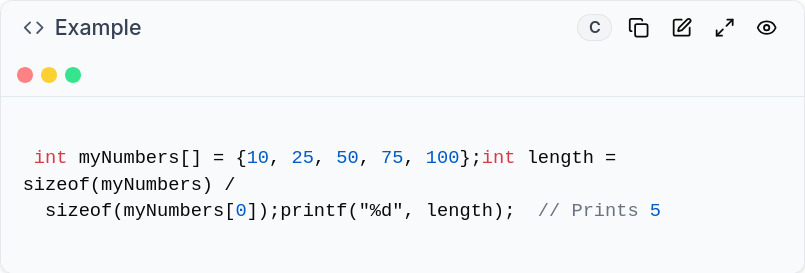
\includegraphics[width=\linewidth]{pre_edit.jpeg} % Replace with your image file
    \caption{Exemple de code interactif avec options d'édition.}
    \label{fig:code_example}
  \end{minipage}\hfill
  \begin{minipage}{0.48\textwidth}
    \centering
    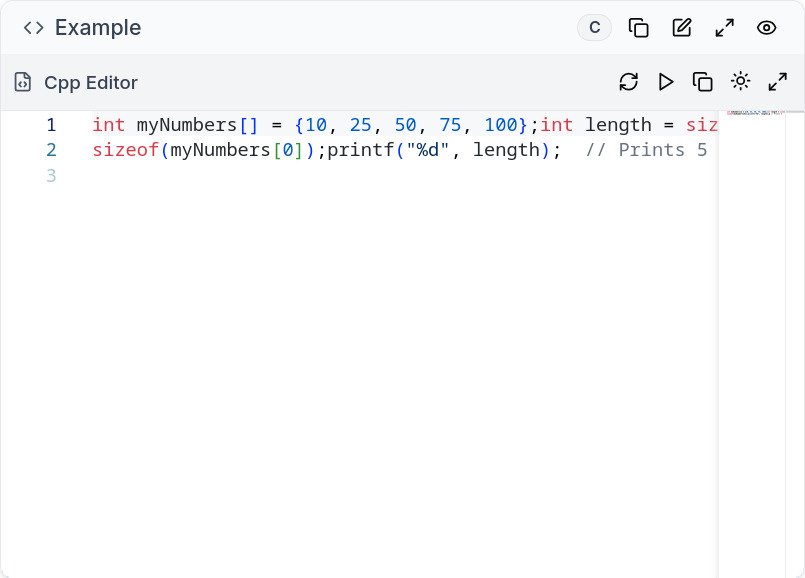
\includegraphics[width=\linewidth]{editmode.jpeg} % Replace with your image file
    \caption{Vue de l'éditeur Cpp avec des fonctionnalités interactives.}
    \label{fig:cpp_editor}
  \end{minipage}
\end{figure}

\begin{figure}[htbp]
  \centering
  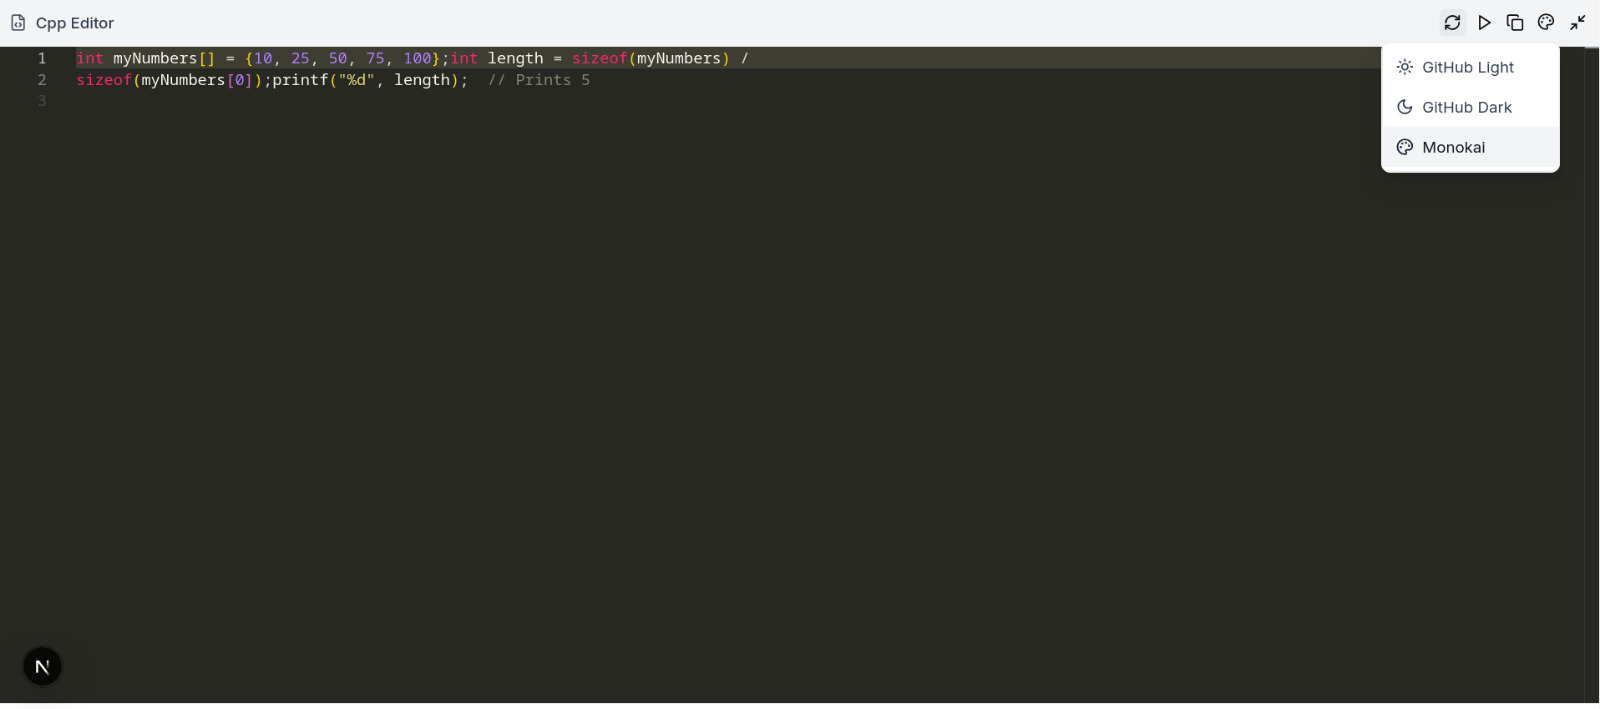
\includegraphics[width=0.5\textwidth]{expended.jpeg} % Replace with your image file
  \caption{Sélection de thèmes pour l'éditeur de code.}
  \label{fig:theme_selection}
\end{figure}

\subsubsection{Ajout d'une Section "Plan du Cours"}
Pour améliorer la navigation au sein des vastes contenus d'apprentissage, une nouvelle section "Plan du Cours" (Course Outline) a été intégrée.
\begin{itemize}
    \item Cette section offre un aperçu structuré des différents modules et leçons d'un cours.
    \item Elle permet une navigation rapide et directe vers des sujets spécifiques, améliorant ainsi l'efficacité de l'apprentissage. (Voir Figure \ref{fig:course_outline}).
\end{itemize}

\begin{figure}[htbp]
  \centering
  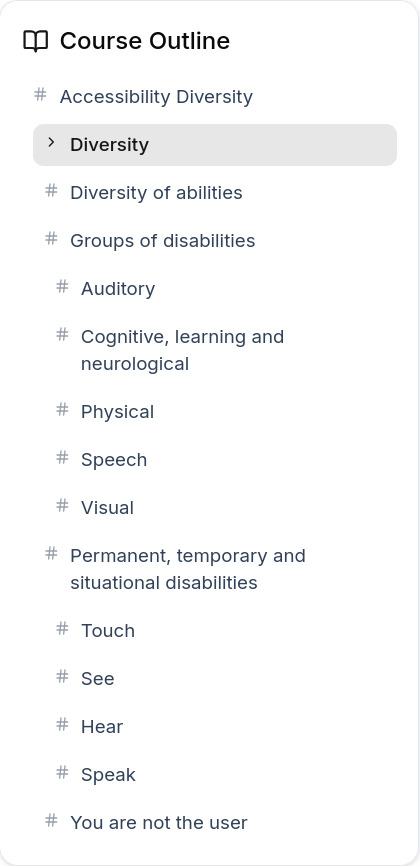
\includegraphics[width=0.4\textwidth]{outline.jpeg} % Replace with your image file
  \caption{Nouvelle section "Plan du Cours" pour une navigation aisée.}
  \label{fig:course_outline}
\end{figure}

\subsubsection{Optimisation de la Barre Latérale de Navigation}
La barre latérale (sidebar) a été améliorée pour aider les utilisateurs à se concentrer sur leurs tâches actuelles :
\begin{itemize}
    \item Un mode "focus" a été implémenté : lorsque l'utilisateur travaille sur un cours spécifique (par exemple, le langage C), les autres catégories de cours peuvent être masquées ou réduites.
    \item Cette fonctionnalité vise à minimiser les distractions et à recentrer l'attention de l'utilisateur sur le contenu pertinent. (Voir Figure \ref{fig:sidebar_context}).
\end{itemize}

\begin{figure}[htbp]
  \centering
  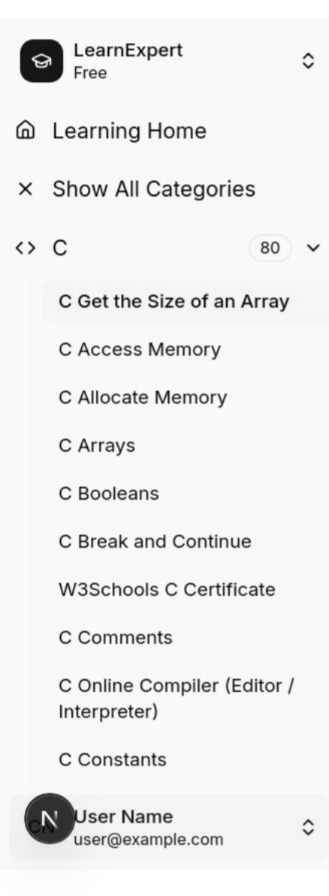
\includegraphics[width=0.35\textwidth]{sidebare2.jpeg} % Replace with your image file
  \caption{Barre latérale améliorée, illustrant la navigation par catégorie.}
  \label{fig:sidebar_context}
\end{figure}

\subsection{Recherche sur l'Optimisation pour les Moteurs de Recherche (SEO) et la Gestion de Site}
La seconde moitié de la journée a été consacrée à l'exploration du domaine du SEO et de la gestion de site.
\begin{itemize}
    \item Conscient que le développement technique seul ne suffit pas à garantir le succès d'une plateforme en ligne, une recherche approfondie a été initiée.
    \item L'objectif est de comprendre les mécanismes permettant d'accroître la visibilité organique du site LearnExpert sur les moteurs de recherche comme Google.
    \item Les sujets abordés incluent les principes fondamentaux du SEO, l'importance des mots-clés, la structure du site, et les bonnes pratiques de gestion de contenu.
    \item Il est prévu de compiler ces recherches et apprentissages dans un rapport dédié une fois une compréhension plus approfondie et une aisance suffisante avec le sujet seront acquises.
\end{itemize}

\subsection{Planification pour le Jour Suivant (Mardi 26 Mai 2025)}
Pour la journée de demain, les objectifs sont les suivants :
\begin{itemize}
  \item Poursuivre l'affinage des éléments UI/UX implémentés aujourd'hui, en intégrant d'éventuels retours ou nouvelles idées.
  \item Approfondir les connaissances en SEO et commencer à esquisser une stratégie SEO initiale pour la plateforme.
  \item Identifier les premières actions SEO concrètes à mettre en œuvre (par exemple, optimisation des balises méta pour les pages clés).
  \item Réévaluer le calendrier de déploiement de la section publique, en tenant compte des récentes améliorations et des bases SEO à établir.
  \item Continuer le développement des fonctionnalités spécifiques pour les utilisateurs premium, conformément au plan de projet global.
\end{itemize}

\section{Conclusion}
Cette première journée de la quatrième semaine a été productive, marquée par des avancées significatives dans l'amélioration de l'interface utilisateur et de l'expérience globale sur la plateforme LearnExpert. L'introduction de fonctionnalités interactives pour les exemples de code, d'un plan de cours structuré et d'une barre latérale optimisée contribue directement à un environnement d'apprentissage plus engageant et efficace. Parallèlement, l'initiation à la recherche en SEO est une étape cruciale pour assurer la découvrabilité et la portée future du projet. Les efforts combinés sur l'UX et le SEO posent des bases solides pour la croissance et le succès de la plateforme.

\end{document}